\chapter{Introduction}
\label{chap:introduction}

\section{Motivation}
Blimps are often used as advertising vehicle. Especially eye-catching are special shaped blimps, e.g. blimps that have the shape of a mascot, car or any other commercial product (see figure \ref{fig:blimps}).
An alternative are conventionally shaped blimps showing imprints or banners.
The arrangement of the actuators for those different shaped blimps varies a lot and needs in general manual adjustment of the control algorithm.
Using some adequate sensors, it would be useful to determine the effect of an actuator on the movement of the blimp automatically.
With such an algorithm, the blimp hull can be manufactured independently on the actuation which just can be attached to the blimp and the controller figures out the effect of its actuators by its own.
This procedure is illustrated in figure \ref{fig:motivation}.

\begin{figure}[hbtp]
\centering
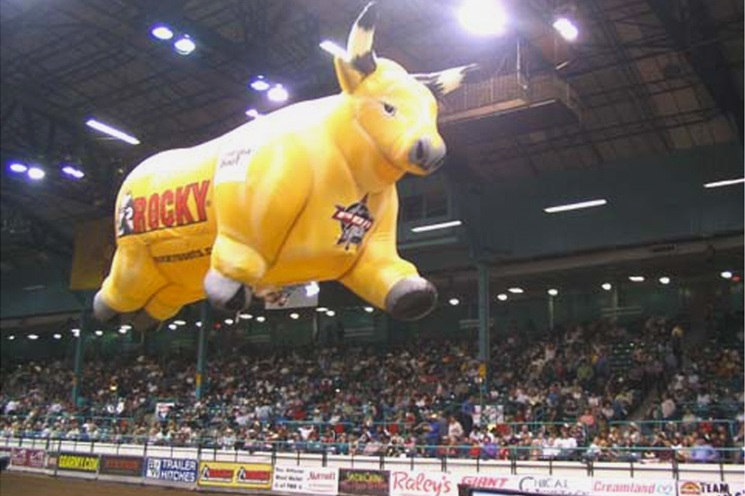
\includegraphics[width=.4\linewidth]{images/CustomBull_Lg.jpg}
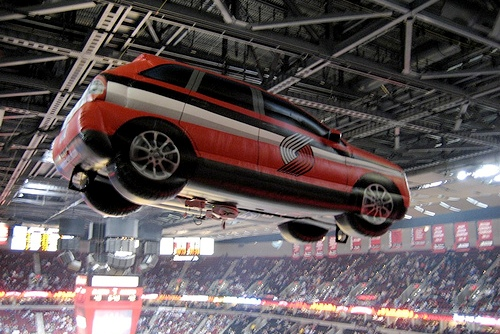
\includegraphics[width=.4\linewidth]{images/CustomCar.jpg}
\caption{Special shaped blimps are used for advertising \citep{rcblimps}.}
\label{fig:blimps}
\end{figure}

\begin{figure}[hbtp]
\centering
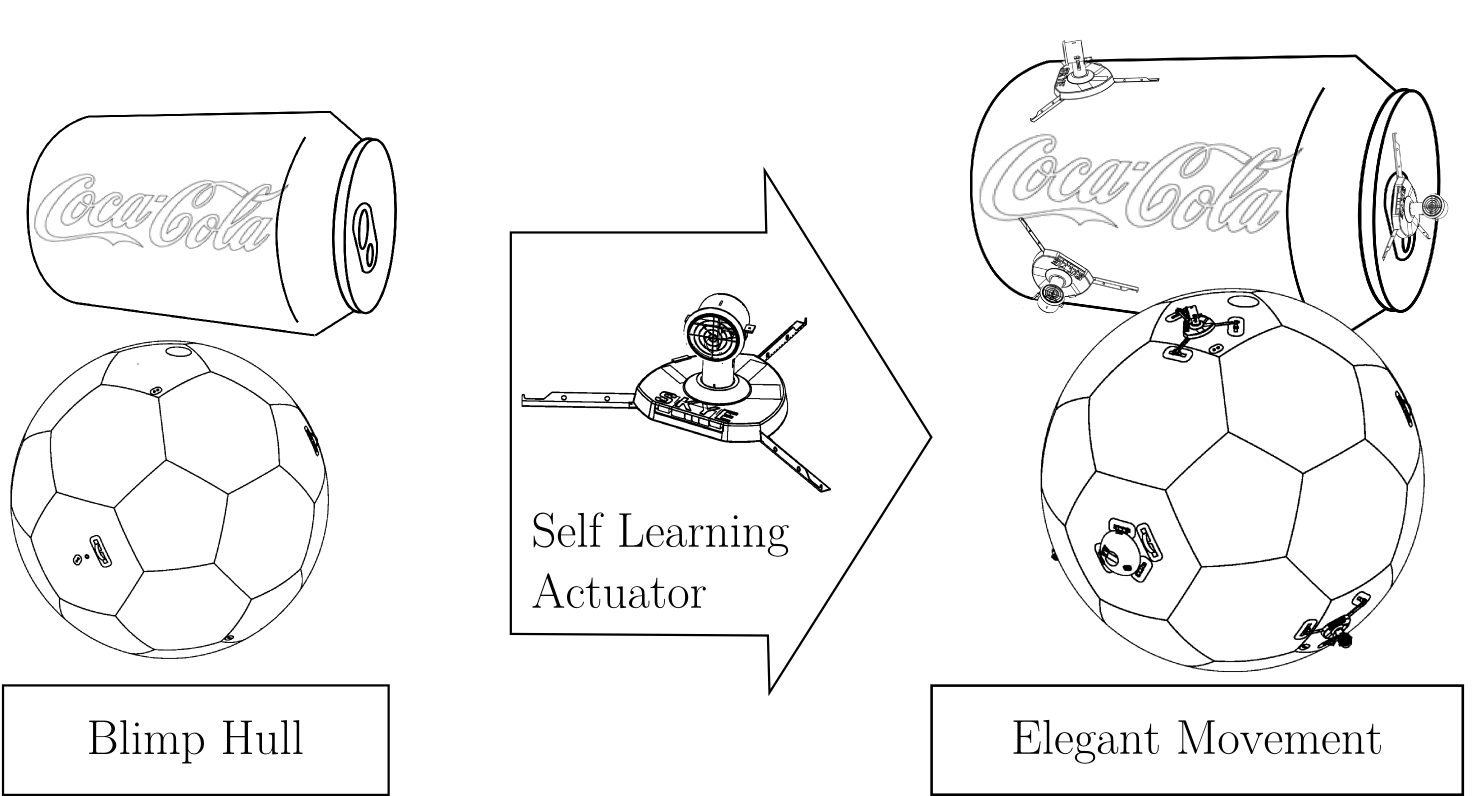
\includegraphics[width=.85\linewidth]{images/motivation.png}
\caption{The goal is to find an algorithm, that allow to take any blimp shape (\textit{left}) and put the actuation units (\textit{center}) on. The actuation configuration is then automatically detected, such that elegant movements can be performed without manual controller adjustments (\textit{right}).}
\label{fig:motivation}
\end{figure}


\section{Configuration Estimation}
This work is on estimation of the actuation configuration for a multi-actuated blimp.
It is motivated on our work on Skye, a spherical and omnidirectional blimp.
Its design and control is described in detail in \citep{Skye2013} and briefly summarized below. \\
Various work on thruster configuration estimation can be found for underwater robot systems.
\citet{Doniec} propose black box model approach.
They calculate an inverse model of the thrusters, i.e. a mapping from a desired rotation and position change of the robot to the thruster commands. After about 40 seconds of random walk, the inverse model is computed as the Moore-Penrose pseudoinverse of the collected input/output data.
\citet{VandeVen2005} show an overview of neural network control of underwater vehicles. \\ 
For our work, we are using a gray box model for the actuation configuration.
A similar batch approach has been chosen by \citep{Shuster1991} for spacecraft sensor alignment estimation.
They determine the rotation vector between multiple star tracker devices. \citet{Bloesch2013} formulated a nonlinear least squares problem to estimate kinematic parameters of a legged robot.
In depth studies using batch optimization have been made for camera-IMU calibration XXXXXXXXX 
! Find citation in AMR book or elsewhere!


\section{Skye System Overview}
The practical part of this work is done with the Skye System \citep{Skye2013}.\\
Skye is a spherical blimp (\cref{fig:frames} right) where the center of gravity coincides with the center of buoyancy.
Four identical actuators (\cref{fig:frames} left) are attached to the hull of Skye in a tetrahedral arrangement.
Each of these actuators can rotate around their z-axis.
Mounted to the rotating part of the actuators there is an impeller which can generate thrust in the XY-plane along the direction it is currently pointed.

\subsection{Coordinate Systems}
This setup gives Skye the ability to move and rotate in all directions with more ore less the same efficiency.\\
In this work we use different coordinate systems for the Skye body and the actuators.\\
The Skye body coordinate system is defined according to the onboard camera as a NED coordinate system. 
When the camera is upright and pointing forward, the body coordinate system has the origin in the center of the spherical blimp and the x-direction points into the direction of the camera, while the z-direction points downwards.\\
Each actuator has its own local coordinate system.
When the actuator is standing on a flat surface, the z-axis is defined to point down.
The coordinate system origin is set to the base of the actuator such that the z-axis coincides with the rotation axe of the actuator.
The x-axis is defined to be pointing in the direction of the thruster when its angle is set to zero.
To put it another way, the thrust-force points in the x-axis direction when the actuator angle is zero.\\
rotation isch als e rechte hand rotation um z definiert?? how to formulate?

\begin{figure}[hbtp]
\centering
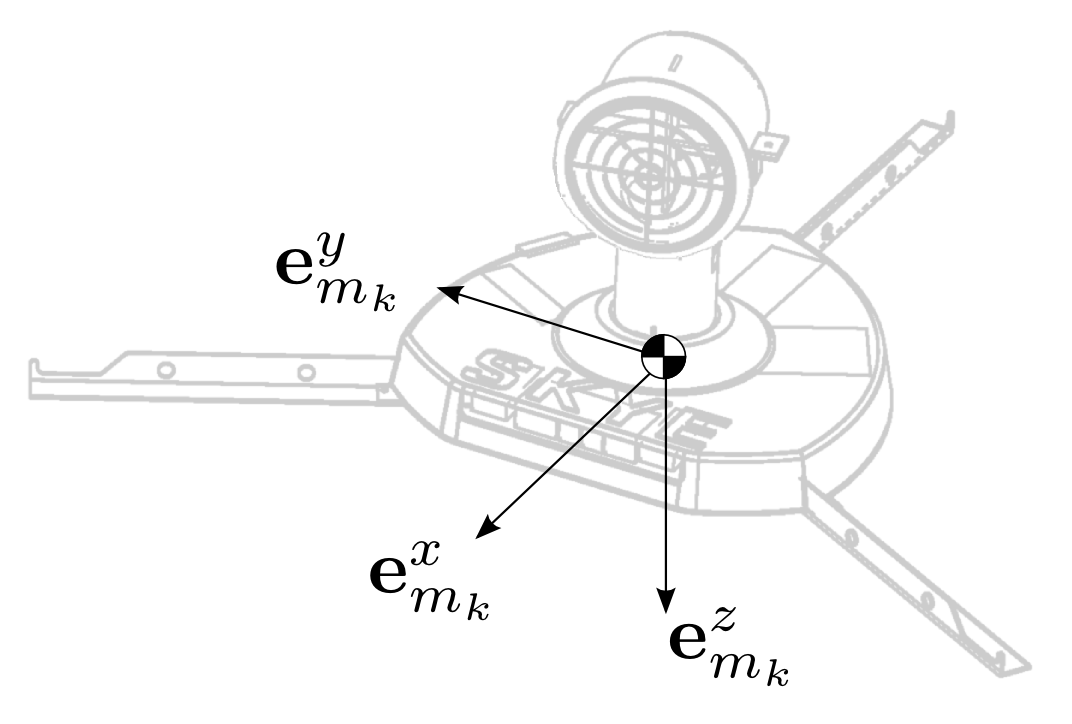
\includegraphics[width=.4\linewidth]{images/motor_frame.png}
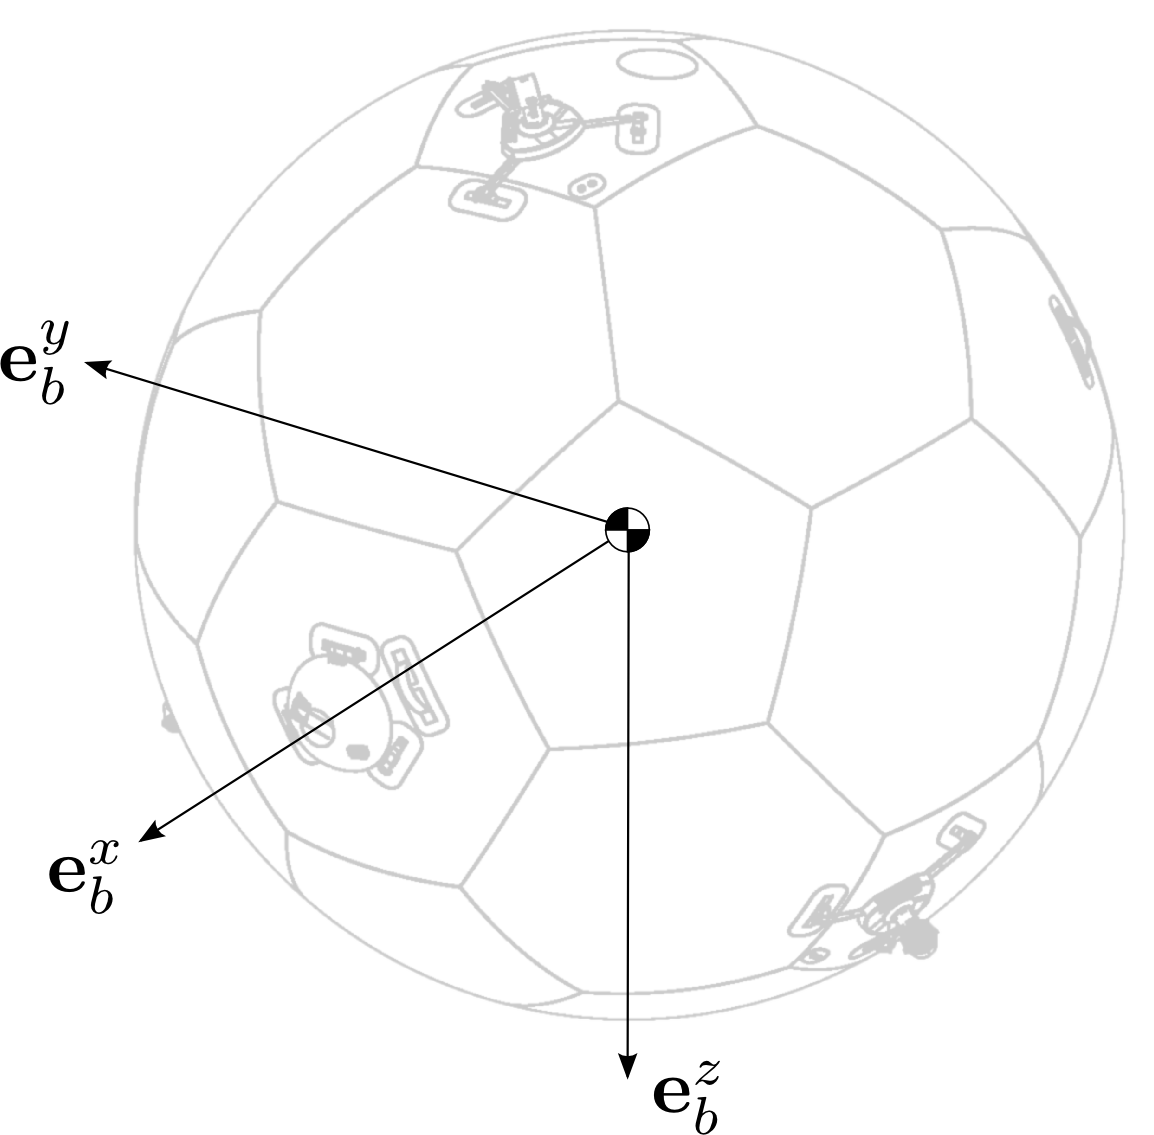
\includegraphics[width=.4\linewidth]{images/blimp_frame.png}
\caption{\textbf{Left}: Motor coordinate frame $m_k$. When the thruster is not rotated, it directs in $\mathbf{e}^x_{m_k}$ direction. $\mathbf{e}^z_{m_k}$ directs to the bottom. \textbf{Right}: Blimp coordinate frame $b$. $\mathbf{e}^x_{b}$ directs to the camera which is mounted at the front. $\mathbf{e}^z_{b}$ directs to the bottom.}
\label{fig:frames}
\end{figure}

\subsection{Hardware and Software}
Skye is based around the Inertial Measurement Unit from the PIXHAWK Research Project (??ref??). 
The firmware of Skye is based on the PX4 autopilot project (??ref??) and augmented with Skye specific features.
To control Skye a QGroundControl (??ref??) based interface is installed on a Laptop which is connected via a XBEE link to the PX4 autopilot.
From there user input is provided with a 3D mouse from 3Dconnexion.

\subsection{Sensors}
Onboard the PX4 autopilot are the sensors used in this work.
While the PX4 autopilot has many sensors the most important sensor for this work is the MPU-6000 Six-Axis (Gyro + Accelerometer) MEMS MotionTracking™ Device.
This sensor measures angular velocities around all three axes of rotation as well as translational acceleration in all three directions. \\
As will be explained later we use mainly the gyro sensor. To get an understanding of the performance of this sensor we measured the noise of the sensor to be about $3.2 \cdot 10^{-4}rad/s$ RMS.

\subsection{Allocation}

\begin{figure}[hbtp]
\centering
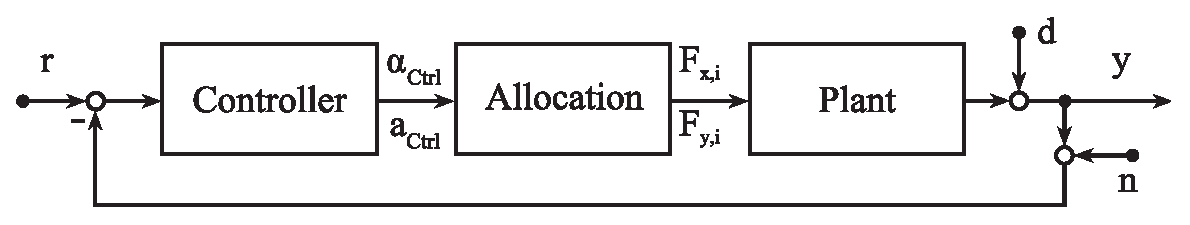
\includegraphics[width=.9\linewidth]{images/system_loop_3.eps}
\caption{Skye control loop.}
\label{fig:system_loop_3}
\end{figure}

The unique thing about Skye is the way controlled flight is achieved. 
\Cref{fig:system_loop_3} shows the control loop of Skye.
Because the actuators of Skye have 8DOF and the flying body has only 6DOF of control, the mapping between the controller output and the actuator inputs is not a unique mapping. (??cite vue??)
This mapping is solved with lagrange with the cost-function set to optimize power consumption of the actuators. See (??ref??) for more details.\\
For this work, the important part about the allocation is that it is derived from the positions and orientations of the motors.

